\documentclass[sigconf]{acmart}

\usepackage{booktabs}
\usepackage{graphicx}
\usepackage{tikz}
\usetikzlibrary{positioning, arrows.meta}

\title{Detecting AI-Generated Code in Introductory CS Submissions: A Multi-Model Fingerprinting Approach}

\author{Uditi Sharma}
\affiliation{
  \institution{New York University Abu Dhabi}
  \department{Computer Science}
}
\email{us2133@nyu.edu}

\begin{abstract}
The availability of large language models has created a real gap in academic integrity enforcement for programming courses, including the Introduction to Computer Science course at NYU Abu Dhabi. MOSS, the standard plagiarism detection tool, works by finding shared substrings between student submissions. It is completely ineffective against AI-generated code because each generation is unique and shares no source document with any other. AI tool adoption among CS students has grown rapidly since 2022, with widespread documented use across computing programs worldwide~\cite{prather2023robots}, yet detection infrastructure has not kept pace.

This project investigates two questions. First, do different AI models leave statistically distinguishable stylistic fingerprints in Introduction to Computer Science assignment code, and do those fingerprints survive prompt-level style variation? Second, can a supervised classifier reliably separate AI-generated submissions from pre-ChatGPT student code on the same assignment? Preliminary results on 423 Connect4 Python implementations generated by 9 models show strong fingerprint persistence (Cohen's d = 0.720, p < 0.001), with 33 of 36 model pairs statistically distinguishable by TF-IDF similarity alone. The second question requires a human baseline of pre-2022 student submissions, which we have obtained from the course instructor.
\end{abstract}

\keywords{AI-generated code detection, academic integrity, code stylometry, authorship attribution, large language models, CS education}

\setcopyright{none}
\settopmatter{printacmref=false}
\renewcommand\footnotetextcopyrightpermission[1]{}

\begin{document}

\maketitle

This report is submitted to NYUAD's capstone repository in fulfillment of NYUAD's Computer Science major graduation requirements.

\section{Introduction}

When a student submits Python code for a Connect4 assignment in the Introduction to Computer Science course at NYU Abu Dhabi, there is currently no reliable way to determine whether they wrote it or generated it with GPT-4o, Claude, or Gemini. MOSS, the standard plagiarism detection tool used in CS departments, works by fingerprinting document content and comparing shared substrings between submissions~\cite{schleimer2003winnowing}. It catches copy-paste between students effectively, but AI-generated code has no source document to share with any other submission. Every generation is unique, and MOSS reports a similarity near zero.

The scale of the problem is real. AI tool adoption among CS students has grown rapidly since 2022, with widespread documented use across institutions and countries~\cite{prather2023robots}, and self-reporting surveys likely undercount actual usage. Instructors who reuse the same assignments year after year are especially exposed, since standard problems like Connect4, Tic-Tac-Toe, and Hangman are exactly the kind that LLMs handle well.

Prior work on detection has made progress but remains narrow. Hoq and Leinonen~\cite{hoq2024detecting} showed that machine learning classifiers can distinguish ChatGPT-generated Java code from human-written code with up to 97\% accuracy on simple Introduction to Computer Science problems. Xu and Sheng~\cite{xu2024detecting} applied perplexity-based methods to code assignments and achieved an average AUC of 0.87. But both studies tested a single model, and none examined whether different models produce distinguishable stylistic signatures. In practice, students use GPT-4o, Claude, Gemini, and other tools, and the programs they submit are far more substantial. It remains an open question whether AI fingerprints hold across models, and whether different models leave distinguishable signatures.

This project addresses two research questions:

\textbf{RQ1 (Multi-model fingerprinting):} Do different AI models leave statistically distinguishable stylistic fingerprints in Introduction to Computer Science assignment code, and do those fingerprints persist across 15 prompt-level style variations?

\textbf{RQ2 (AI vs. human detection):} Can a supervised classifier reliably separate AI-generated submissions from pre-ChatGPT student code on the same assignment?

RQ1 is the methodological prerequisite for RQ2. If AI models do not leave statistically distinguishable fingerprints in their code, there is no model-identifying signal for a classifier to learn. Confirming RQ1 provides evidence that features such as TF-IDF similarity, AST structure, and CodeBERT embeddings carry model-identifying information --- and those same features become the inputs to the RQ2 classifier. RQ1 is answered with data already collected and analyzed. RQ2 is planned for Fall 2026 once the pre-2022 human baseline submissions are integrated into the pipeline.

\section{Related Work}

\textbf{Detecting ChatGPT in Introduction to Computer Science Courses (Hoq and Leinonen, SIGCSE 2024)~\cite{hoq2024detecting}.} The closest prior work in the educational setting. They trained classifiers on ChatGPT-generated and human-written Java solutions to simple Introduction to Computer Science problems. Their best model achieved 97\% accuracy. However, they tested only GPT-3.5 and produced binary labels. Binary labels are problematic for academic integrity cases where a probability score with interpretable evidence is far more defensible.

\textbf{AIGCode (Xu and Sheng, AAAI 2024)~\cite{xu2024detecting}.} This paper framed the problem identically to ours: detecting AI-generated code in academic submissions. Their method uses targeted masking and CodeBERT fill-in to compute perplexity scores, achieving AUC 0.87 against text-davinci-003. They used competitive programming problems from CodeNet rather than actual student submissions, and tested only one model.

\textbf{DetectCodeGPT (Shi et al., ICSE 2025)~\cite{shi2025between}.} The most rigorous zero-shot approach published so far. Their NPR metric (Normalized Perturbed Log Rank) exploits the fact that machine-generated code is more locally optimal under the model that produced it. They achieved AUROC 0.93 in some settings. However, they only tested open-source code models such as Incoder, StarCoder, and CodeLlama, and explicitly did not test GPT-4o or Claude.

\textbf{GPTSniffer (Nguyen et al., JSS 2024)~\cite{nguyen2024snippet}.} Fine-tuned CodeBERT as a binary classifier, achieving near-perfect precision when training used paired samples (human and AI solving the same problem), compared to F1 around 0.73 with unpaired data. This validates our paired training design for RQ2. They tested only GPT-3.5 on GitHub code snippets, not assignment submissions.

\textbf{AIGC detectors fail on code (Wang et al., 2023)~\cite{wang2023evaluating}.} Systematically evaluated six existing AIGC detectors on code. All performed significantly worse on code than on natural language text, and cross-domain generalization remained limited even after fine-tuning. This motivates assignment-specific detectors over general-purpose tools.

\textbf{Embedding and classifier approaches (Oedingen et al., AI 2024)~\cite{oedingen2024chatgpt}.} Benchmarked multiple detection methods including Random Forest, XGBoost, and DNN on embedding features. Embedding plus DNN achieved 98\% accuracy; humans alone cannot detect AI code at above-chance rates. Their results support our classifier choice for RQ2.

\textbf{CodeBERT (Feng et al., EMNLP 2020)~\cite{feng2020codebert}.} A RoBERTa-based model pre-trained on natural language and code pairs from CodeSearchNet. We use CodeBERT's [CLS] token embeddings as semantic features. It was designed for NL-to-code retrieval, not authorship analysis. Our use is an empirical extension, and we report it as such.

\section{Methodology}

\subsection{Dataset Construction}

We built a controlled dataset of 423 Connect4 Python implementations generated by 9 LLMs across two generations. Connect4 is a standard assignment in the Introduction to Computer Science course at NYU Abu Dhabi, requiring a 6x7 board, two-player logic with checkers X and O, win detection in four directions, input validation, and screen-clearing between turns. Using a specific assignment with concrete requirements allows direct comparison across models and, eventually, with human submissions. This study focuses on Connect4 as the primary target; the methodology is designed to generalize to other standard assignments in the same course, and will be extended to two additional assignments in Fall 2026.

\begin{table}[h]
\caption{Dataset: 423 AI-generated Connect4 implementations}
\label{tab:dataset}
\begin{tabular}{lrr}
\toprule
Model & Era & N \\
\midrule
GPT-4o            & 2024 & 70 \\
GPT-4o Mini       & 2024 & 50 \\
Claude Sonnet 3.5 & 2024 & 50 \\
Gemini 2.0 Flash  & 2024 & 50 \\
Llama 3.1 70B     & 2024 & 50 \\
Claude Opus 4.5   & 2025 & 28 \\
o4-mini           & 2025 & 43 \\
Claude Sonnet 4.6 & 2025 & 41 \\
Claude Opus 4.6   & 2025 & 41 \\
\midrule
\textbf{Total}    &      & \textbf{423} \\
\bottomrule
\end{tabular}
\end{table}

Each model was prompted under 15 distinct style instructions, listed in Table~\ref{tab:styles}. These span a range of surface-level variations that a student might plausibly apply when trying to make AI-generated code look more personal: altering verbosity, comment density, naming conventions, and structural organization. The choice to vary prompts systematically is what allows us to test fingerprint \emph{persistence} rather than mere fingerprint \emph{existence}. The average file is 110 lines long.

\begin{table}[h]
\caption{The 15 style instructions appended to the base prompt}
\label{tab:styles}
\small
\begin{tabular}{cl}
\toprule
\# & Style instruction \\
\midrule
1  & Simple, beginner-friendly style with clear variable names \\
2  & Compact style, minimizing lines of code \\
3  & Detailed inline comments explaining every section \\
4  & Professional style following PEP\,8 strictly \\
5  & Descriptive function names and minimal comments \\
6  & As concise as possible, avoiding any redundancy \\
7  & Teaching style, as if explaining to a Python learner \\
8  & Focus on readability over brevity \\
9  & Only basic Python features a first-year student would know \\
10 & Modular structure, breaking everything into small functions \\
11 & Extensive docstrings for every function \\
12 & Functional style, avoiding global variables where possible \\
13 & Prioritizing correctness and clarity over elegance \\
14 & Minimal whitespace and short variable names \\
15 & Straightforward, no-frills style \\
\bottomrule
\end{tabular}
\end{table}

Two additional models (Gemini 2.5 Flash and Pro) were excluded after we found they consistently generated truncated 20-line files. Their internal reasoning tokens consumed the 3,000-token generation budget before any actual code was output. This is a reproducible limitation of applying thinking models to code generation with a fixed token budget.

Data was generated in two phases. The 2024 models were generated via OpenRouter. The 2025 models were generated via NYU's Portkey AI Gateway. Each file has a provenance header recording model, timestamp, style index, token counts, and MD5 hash.

\subsection{Feature Extraction}

We extract three complementary representations from each file.

\textbf{Lexical features (TF-IDF).} We tokenize each file using Python's built-in tokenizer to produce unigrams and bigrams of token types, keywords, and identifiers. TF-IDF vectors capture vocabulary habits: which variable names a model prefers, how it structures loops, whether it uses list comprehensions.

\textbf{Structural features (AST-based).} We parse each file into an Abstract Syntax Tree and extract: function count, cyclomatic complexity, maximum nesting depth, comment density, average function length, and use of list comprehensions and lambda expressions. These capture code organization at a structural level independent of vocabulary.

\textbf{Semantic features (CodeBERT).} We pass each file through CodeBERT and extract the [CLS] token embedding as a 768-dimensional vector~\cite{feng2020codebert}. This is an empirical probe of whether semantic similarity in CodeBERT's embedding space correlates with model identity.

Figure~\ref{fig:pipeline} shows the full analysis pipeline.

\begin{figure}[h]
\centering
\resizebox{\columnwidth}{!}{%
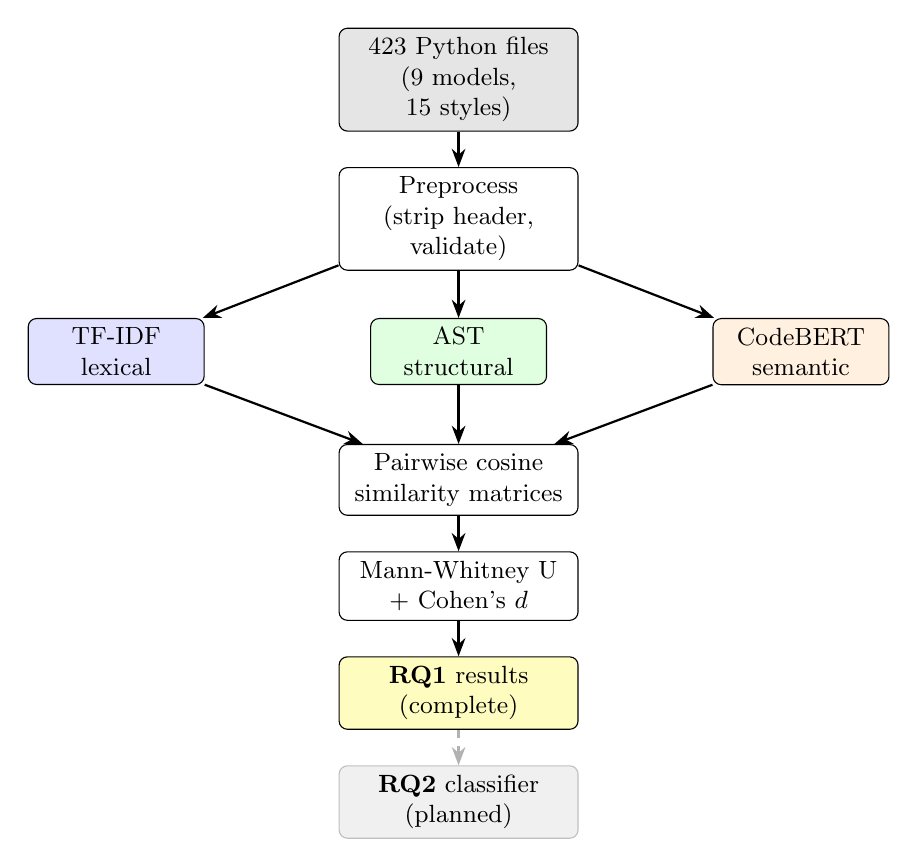
\begin{tikzpicture}[
  box/.style={draw, rectangle, rounded corners=3pt, text centered,
              text width=2.8cm, minimum height=0.7cm, font=\small},
  feat/.style={draw, rectangle, rounded corners=3pt, text centered,
               text width=2.0cm, minimum height=0.7cm, font=\small},
  arr/.style={-{Stealth}, thick},
  darr/.style={-{Stealth}, thick, dashed, gray!60}
]
  \node[box, fill=gray!20]                              (inp) {423 Python files\\(9 models, 15 styles)};
  \node[box, below=0.45cm of inp]                       (pre) {Preprocess\\(strip header, validate)};
  \node[feat, below left=0.6cm and 1.7cm of pre,  fill=blue!12]   (tf)  {TF-IDF\\lexical};
  \node[feat, below=0.6cm of pre,                fill=green!12]  (ast) {AST\\structural};
  \node[feat, below right=0.6cm and 1.7cm of pre, fill=orange!12] (cb)  {CodeBERT\\semantic};
  \node[box, below=2.2cm of pre]                        (sim) {Pairwise cosine\\similarity matrices};
  \node[box, below=0.45cm of sim]                       (mw)  {Mann-Whitney U\\+ Cohen's $d$};
  \node[box, below=0.45cm of mw,  fill=yellow!25]       (rq1) {\textbf{RQ1} results\\(complete)};
  \node[box, below=0.45cm of rq1, fill=gray!12, draw=gray!50] (rq2) {\textbf{RQ2} classifier\\(planned)};
  \draw[arr] (inp) -- (pre);
  \draw[arr] (pre) -- (tf);
  \draw[arr] (pre) -- (ast);
  \draw[arr] (pre) -- (cb);
  \draw[arr] (tf)  -- (sim);
  \draw[arr] (ast) -- (sim);
  \draw[arr] (cb)  -- (sim);
  \draw[arr] (sim) -- (mw);
  \draw[arr] (mw)  -- (rq1);
  \draw[darr](rq1) -- (rq2);
\end{tikzpicture}
}
\caption{Analysis pipeline. The three feature representations are computed in parallel and merged for pairwise similarity analysis. RQ2 (dashed) is planned for Fall 2026.}
\label{fig:pipeline}
\end{figure}

\subsection{Similarity Analysis (RQ1)}

For each feature type, we compute an $N \times N$ pairwise cosine similarity matrix. We separate pairwise scores into two groups: within-model pairs (same model generated both files) and between-model pairs (different models). We compare distributions using the Mann-Whitney U test, a non-parametric test that makes no assumption of normality, and measure effect size with Cohen's $d$. We also compare per-model within-group distributions pairwise to determine which model pairs are statistically distinguishable. Critically, within-model pairs are drawn from files generated under \emph{different} style conditions; a consistently high within-model similarity therefore directly tests whether fingerprints survive prompt-level variation, not merely that a model produces internally consistent output at a fixed prompt.

\subsection{Classification (RQ2, planned Fall 2026)}

\textbf{Human baseline similarity analysis.} Before training any classifier, we will run the identical TF-IDF pairwise similarity analysis on the pre-2022 student submissions. The RQ2 classifier rests on the assumption that human-written code occupies a more diffuse region of feature space than AI-generated code --- that is, human submissions are less internally consistent with each other than a single model's outputs are with themselves. We will verify this assumption directly by computing within-human cosine similarity and comparing it against the per-model distributions from RQ1 using the same Mann-Whitney U and Cohen's $d$ framework. If within-human similarity is not significantly lower than within-model similarity, the feature space does not support clean separation and the classifier architecture would need to be reconsidered. If it is --- as expected --- this analysis produces a human fingerprint distribution that can be visualized alongside the 9 AI model distributions as a pre-classifier justification for why RQ2 is feasible.

The pre-ChatGPT student Connect4 submissions are in hand from the course instructor and will be integrated in Fall 2026. Because the number of AI-generated files will exceed human submissions, we will address class imbalance explicitly via class-weighted training and decision-threshold tuning rather than synthetic oversampling, which can inflate held-out validation performance. Cross-validation folds will be stratified on source (AI vs.\ human) to maintain balanced class representation across folds. Within the AI partition, we additionally verify that each fold samples from all 9 models and all 15 style conditions, so that no single model's fingerprint or style variant dominates any fold.

The classifier output will be a probability score rather than a binary label. Binary labels are inappropriate for academic integrity cases: a false accusation is costly to a student and potentially actionable against an institution. We will tune the decision threshold to prioritize precision over recall, and we will report full precision-recall curves so that instructors can select an operating point based on their institution's risk tolerance. We will evaluate both Random Forest and XGBoost and report which feature types (TF-IDF, AST, CodeBERT, or a combination) contribute most to separability.

A secondary analysis will investigate \textbf{model attribution}: rather than asking only whether a submission is AI-generated, we ask \emph{which} model it most resembles. Using the per-model fingerprints established in RQ1, each submission can be compared against the nine model fingerprint distributions via nearest-neighbor similarity. If a student submission clusters near GPT-4o's fingerprint rather than the human cluster, that provides richer and more actionable evidence than a binary flag alone. This attribution analysis will be conducted if post-2022 student submissions (where AI use was possible) are available from the course instructor, allowing us to observe whether real submissions cluster near specific model fingerprints without requiring ground-truth labels.

\section{Evaluation}

\subsection{Hypotheses}

\textbf{H1 (RQ1 --- overall fingerprint):} Within-model TF-IDF cosine similarity is significantly higher than between-model similarity, indicating that AI models produce code with consistent stylistic patterns.\\
\textit{Status: Confirmed. Cohen's $d = 0.720$, $p < 0.001$.}

\textbf{H2 (RQ1 --- pairwise distinguishability):} Most pairwise model combinations are statistically distinguishable by their stylistic fingerprints across 15 prompt-level style variations.\\
\textit{Status: Confirmed. 27 of 36 pairs significant at $p < 0.001$; 33 of 36 significant at $p < 0.05$.}

\textbf{H3 (RQ2 --- AI vs.\ human, planned):} A classifier trained on TF-IDF, AST, and CodeBERT features can distinguish AI-generated Connect4 code from pre-ChatGPT student submissions with AUC $\geq 0.90$.\\
\textit{Status: To be evaluated Fall 2026.}

\textbf{H4 (RQ2 --- human baseline diversity, planned):} Within-human TF-IDF cosine similarity is significantly lower than the mean within-model similarity observed across the 9 AI models (0.793), indicating that pre-ChatGPT student submissions occupy a more diffuse region of the feature space. If confirmed, this validates the premise that AI-generated and human-written code are separable in the same feature space used for RQ1 --- before any classifier is trained.\\
\textit{Status: To be evaluated Fall 2026.}

\subsection{Preliminary Results (RQ1)}

\textbf{Overall fingerprint signal.} Across all 423 files, within-model TF-IDF cosine similarity (mean 0.793) significantly exceeds between-model similarity (mean 0.719). The mean difference is 0.074, Cohen's $d = 0.720$, and $p < 0.001$ (Mann-Whitney U, effectively zero). This is a medium-to-large effect: the within-model and between-model distributions are meaningfully separated.

\begin{figure}[h]
  
\includegraphics[width=\columnwidth]{similarity_distribution_tfidf}
  \caption{Distribution of within-model vs.\ between-model TF-IDF cosine similarity across 423 files. The within-model distribution (right) is clearly shifted higher, confirming the fingerprint signal.}
  \label{fig:sim_dist}
\end{figure}

\begin{figure}[h]
  
\includegraphics[width=\columnwidth]{similarity_heatmap_tfidf}
  \caption{Pairwise mean TF-IDF cosine similarity across all 9 models (423 files). Diagonal entries represent within-model similarity. GPT-4o Mini and Claude Sonnet 3.5 show the highest internal consistency; Claude Sonnet 4.6 shows the most variation.}
  \label{fig:heatmap}
\end{figure}

\textbf{Per-model consistency.} Table~\ref{tab:similarity} shows within-model similarity varies meaningfully across models. GPT-4o Mini has the highest internal consistency (mean 0.833, std 0.071). Claude Sonnet 4.6 shows the most variation (mean 0.710, std 0.165), the lowest mean of all 9 models by a clear margin. A secondary pattern emerges across generations: 2024-era model standard deviations range from 0.062 to 0.118, while 2025-era models are more mixed --- o4-mini is tightly consistent (std 0.073), comparable to GPT-4o Mini, whereas Claude Sonnet 4.6 (std 0.165) is considerably more variable than its 2024 counterpart Claude Sonnet 3.5 (std 0.062). Whether this reflects deliberate output diversity in newer training runs or increased sensitivity to prompt phrasing is a secondary question we flag for future analysis. We note that Claude Opus 4.5's smaller sample (n = 28) may reduce the precision of its mean and std estimates relative to models with 41--70 files.

\begin{table}[h]
\caption{Within-model TF-IDF cosine similarity (423 files)}
\label{tab:similarity}
\begin{tabular}{llrr}
\toprule
Model & Era & Mean & Std \\
\midrule
GPT-4o Mini       & 2024 & 0.833 & 0.071 \\
Claude Sonnet 3.5 & 2024 & 0.819 & 0.062 \\
Claude Opus 4.5   & 2025 & 0.804 & 0.148 \\
o4-mini           & 2025 & 0.800 & 0.073 \\
GPT-4o            & 2024 & 0.800 & 0.106 \\
Claude Opus 4.6   & 2025 & 0.793 & 0.109 \\
Gemini 2.0 Flash  & 2024 & 0.780 & 0.118 \\
Llama 3.1 70B     & 2024 & 0.772 & 0.113 \\
Claude Sonnet 4.6 & 2025 & 0.710 & 0.165 \\
\bottomrule
\end{tabular}
\end{table}

\textbf{Distinguishable pairs.} Of 36 pairwise model comparisons, 27 are highly significant ($p < 0.001$), 6 are significant at $p < 0.05$, and 3 are not distinguishable by TF-IDF alone: GPT-4o Mini vs.\ Claude Opus 4.5 ($p = 0.210$), Claude Opus 4.5 vs.\ Claude Sonnet 3.5 ($p = 0.467$), and Gemini 2.0 Flash vs.\ Llama 3.1 70B ($p = 0.314$). The two non-significant Anthropic pairs are consistent with the hypothesis that same-company models share architectural patterns that produce lexically similar code; however, we cannot rule out a sample-size confound, since Claude Opus 4.5 has only 28 files compared to 41--70 for other models, which reduces statistical power in comparisons involving that model. The Gemini--Llama overlap is harder to explain by lineage and may reflect coincidental lexical convergence on the Connect4 problem structure rather than shared architecture. Both classes of non-significant pairs motivate including structural and semantic features in the Fall 2026 classifier, where structural invariants (nesting depth, function count) and CodeBERT embeddings may recover separability that lexical features alone cannot achieve.

\begin{figure}[h]
  
\includegraphics[width=\columnwidth]{model_comparison_tfidf}
  \caption{Within-model TF-IDF cosine similarity for each of the 9 models (mean $\pm$ 1 std), sorted by mean. The dashed red line marks the overall between-model mean (0.719). Every model's within-model mean exceeds this baseline; GPT-4o Mini is most internally consistent (0.833) while Claude Sonnet 4.6 shows the widest spread (0.710, std 0.165).}
  \label{fig:per_model}
\end{figure}

\subsection{Threats to Validity}

\textbf{Assignment specificity.} All AI files were generated for a single assignment (Connect4). Fingerprints that distinguish models on Connect4 may not transfer to structurally different problems. We treat this as a deliberate design choice rather than a limitation: the paper argues for assignment-specific detectors that exploit the fact that instructors reuse standard assignments annually, and cross-assignment generalizability is a separate question for future work.

\textbf{Human baseline cleanliness.} We assume pre-November 2022 student submissions are free of AI-generated code. In practice, students may have shared code with peers, copied from GitHub repositories, or submitted prior-year solutions. Such contamination would make the human class noisier and inflate the apparent difficulty of RQ2 classification. We will document the instructor's data collection context and flag statistically anomalous submissions (unusually high similarity to the AI distribution) for manual review before training.

\textbf{Sample size for RQ2 classification.} The current 423-file dataset is adequate for the pairwise similarity analysis in RQ1 but is small for training and cross-validating a multi-class classifier in RQ2. Cross-validation folds must be stratified across source (AI vs.\ human), 9 models, and 15 style conditions simultaneously; with 423 AI files, several folds may contain as few as 3--5 files per model per style condition. Prior work achieving high accuracy (Hoq et al., GPTSniffer) used similarly small datasets, but generalization claims are more defensible with larger samples. We plan to expand the AI dataset to approximately 6,000 files per assignment (roughly 667 per model) across all three assignments in Fall 2026 before training the RQ2 classifier, budget permitting.

\textbf{Lexical feature coverage.} TF-IDF captures vocabulary habits but is insensitive to semantic paraphrasing: two files with different variable names but identical algorithmic structure would appear dissimilar under TF-IDF. This is the primary motivation for including AST structural features and CodeBERT semantic embeddings. The three non-significant model pairs identified under TF-IDF are the first targets for re-evaluation once all feature types are incorporated.

\section{Project Timeline}

This proposal covers work completed in Spring 2026. The capstone will be completed in Fall 2026.

\begin{table}[h]
\caption{Completed work, Spring 2026}
\label{tab:timeline}
\begin{tabular}{ll}
\toprule
Task & Status \\
\midrule
AI dataset (423 files, 9 models) & Complete \\
Feature extraction: TF-IDF, AST, CodeBERT & Complete \\
Similarity analysis and hypothesis testing (RQ1) & Complete \\
Capstone proposal & Complete \\
\bottomrule
\end{tabular}
\end{table}

\textbf{Fall 2026:}
\begin{itemize}
  \item Expand AI dataset to $\sim$6,000 files per assignment ($\sim$667 per model) across all three assignments for sufficient classifier training power
  \item Integrate pre-2022 student Connect4 submissions (in hand from course instructor) as the human baseline
  \item Run human baseline similarity analysis (same TF-IDF pipeline as RQ1) to verify H4 before classifier training
  \item Train and evaluate Random Forest and XGBoost classifier for RQ2
  \item Incorporate CodeBERT embeddings into the full classifier pipeline
  \item Finalize RQ2 evaluation across all feature types and style variations
  \item Extend dataset and analysis to two additional assignments from the Introduction to Computer Science course at NYU Abu Dhabi
  \item Write, submit, and defend the full capstone paper (target: SIGCSE 2027 or EDM 2027)
\end{itemize}

\section{Budget}

\textbf{Data collection (expansion, \$1,530):} The current dataset of 423 AI-generated files covers Connect4 only and is sufficient for RQ1 fingerprinting analysis. Fall 2026 requires 6,000 files per assignment across all three Introduction to Computer Science assignments ($\sim$667 per model), providing adequate statistical power for the RQ2 classifier. At this scale, 5-fold cross-validation yields $\sim$534 training and $\sim$133 test files per model per fold --- enough to hold out a credible test set while retaining sufficient training data. All three assignments are budgeted at the same scale to enable direct cross-assignment comparison of fingerprint strength.

The 423 existing files were generated through NYU's Portkey AI Gateway and OpenRouter at no cost. Continued Portkey access is not guaranteed for Fall 2026; if unavailable, files must be generated via direct commercial API calls. Table~\ref{tab:budget} shows estimated costs per assignment at current public rates (500 input tokens and 2,500 output tokens per file, matching the observed Connect4 average).

\begin{table}[h]
\caption{Estimated API cost per assignment ($\sim$667 files per model, 6,000 total)}
\label{tab:budget}
\small
\begin{tabular}{lrrr}
\toprule
Model & Input \$/1M & Output \$/1M & Est.\ cost \\
\midrule
GPT-4o            & \$2.50  & \$10.00 & \$18 \\
GPT-4o Mini       & \$0.15  & \$0.60  & \$1  \\
Claude Sonnet 3.5 & \$3.00  & \$15.00 & \$26 \\
Claude Sonnet 4.6 & \$3.00  & \$15.00 & \$26 \\
Claude Opus 4.5   & \$15.00 & \$75.00 & \$130 \\
Claude Opus 4.6   & \$15.00 & \$75.00 & \$130 \\
Gemini 2.0 Flash  & \$0.08  & \$0.30  & \$1  \\
Llama 3.1 70B     & \multicolumn{2}{c}{\$0.52/1M (flat)} & \$1  \\
o4-mini           & \$1.10  & \$4.40  & \$8  \\
\midrule
\textbf{Subtotal (1 assignment)} & & & \textbf{\$340} \\
\textbf{$\times$ 3 assignments}  & & & \textbf{\$1,020} \\
50\% contingency                 & & & \$510 \\
\midrule
\textbf{Total requested} & & & \textbf{\$1,530} \\
\bottomrule
\end{tabular}
\end{table}

Costs are dominated by the two Opus models (\$260 per assignment, \$780 across three). If Portkey access continues into Fall 2026, this budget will not be spent; it is a contingency against losing university-subsidized API access. We request \textbf{\$1,530} to cover all three assignments at uniform scale.

\textbf{Compute (\$0):} Feature extraction, TF-IDF vectorization, AST parsing, CodeBERT inference, and classifier training all run on personal hardware or NYU HPC (free for registered students). No cloud compute budget is required.

\textbf{Total budget requested: \$1,530.}

\section{Conclusion}

This project makes three contributions beyond prior work. It is the first multi-model fingerprinting study on Introduction to Computer Science assignment code, covering 9 models across two LLM generations (2024 and 2025), while all prior work tested a single model. It uses a verified pre-ChatGPT student baseline rather than GitHub code as a proxy for human writing, which better matches the actual detection target in educational settings. And it operates on realistic-length Introduction to Computer Science implementations (average 110 lines), while prior work either used short code snippets of roughly 10 lines (GPTSniffer on GitHub), competitive programming problems rather than course assignments (Xu and Sheng), or a single language and model on Introduction to Computer Science programs without multi-model comparison (Hoq et al.).

Preliminary results on RQ1 show strong and statistically significant fingerprints across most model pairs. The full AI vs.\ human classification task (RQ2), using pre-2022 student submissions now in hand, will be completed in Fall 2026. It will complete the pipeline from ``can we tell models apart?'' to ``can we tell AI from a real student?''

Beyond binary detection, the per-model fingerprints established in RQ1 open a further question: can we attribute a suspicious submission to a specific model? If a student submission clusters near GPT-4o's fingerprint distribution rather than the human cluster, an instructor receives not just a flag but a specific hypothesis about which tool was used. This model attribution angle --- nearest-neighbor comparison against established fingerprints rather than binary classification --- is a natural extension of the RQ1 findings and distinguishes this work further from prior single-model detection approaches.

\bibliographystyle{ACM-Reference-Format}

\begin{thebibliography}{9}

\bibitem{schleimer2003winnowing}
S.~Schleimer, D.~S.~Wilkerson, and A.~Aiken.
\newblock Winnowing: Local algorithms for document fingerprinting.
\newblock In \textit{Proc. ACM SIGMOD}, pp. 76--85, 2003.

\bibitem{prather2023robots}
J.~Prather, P.~Denny, J.~Leinonen, B.~A.~Becker, I.~Albluwi, M.~Craig, H.~Keuning, N.~Kiesler, T.~Kohn, A.~Luxton-Reilly, S.~MacNeil, A.~Petersen, R.~Pettit, B.~N.~Reeves, and J.~Savelka.
\newblock The robots are here: Navigating the generative AI revolution in computing education.
\newblock In \textit{Proc. ACM ITiCSE-WGR}, 2023.
\newblock \url{https://doi.org/10.1145/3623762.3633499}

\bibitem{hoq2024detecting}
M.~Hoq, Y.~Shi, J.~Leinonen, D.~Babalola, C.~Lynch, T.~Price, and B.~Akram.
\newblock Detecting ChatGPT-generated code submissions in a CS1 course.
\newblock In \textit{Proc. ACM SIGCSE}, 2024.
\newblock \url{https://dl.acm.org/doi/10.1145/3626252.3630826}

\bibitem{xu2024detecting}
Z.~Xu and V.~S.~Sheng.
\newblock Detecting AI-generated code assignments using perplexity of large language models.
\newblock In \textit{Proc. AAAI}, vol. 38, no. 21, pp. 23155--23162, 2024.
\newblock \url{https://doi.org/10.1609/aaai.v38i21.30361}

\bibitem{shi2025between}
Y.~Shi, H.~Zhang, C.~Wan, and X.~Gu.
\newblock Between lines of code: Unraveling the distinct patterns of machine and human programmers.
\newblock In \textit{Proc. ICSE}, 2025.
\newblock arXiv:2401.06461

\bibitem{nguyen2024snippet}
P.~T.~Nguyen, J.~Di~Rocco, C.~Di~Sipio, R.~Rubei, D.~Di~Ruscio, and M.~Di~Penta.
\newblock {GPTSniffer}: A {CodeBERT}-based classifier to detect source code written by {ChatGPT}.
\newblock \textit{Journal of Systems and Software}, vol. 214, 2024.
\newblock \url{https://doi.org/10.1016/j.jss.2024.112059}

\bibitem{wang2023evaluating}
J.~Wang, S.~Liu, X.~Xie, and Y.~Li.
\newblock Evaluating AIGC detectors on code content.
\newblock arXiv:2304.05193, 2023.

\bibitem{oedingen2024chatgpt}
M.~Oedingen, R.~C.~Engelhardt, R.~Denz, M.~Hammer, and W.~Konen.
\newblock ChatGPT code detection: Techniques for uncovering the source of code.
\newblock \textit{AI (MDPI)}, vol. 5, no. 3, pp. 1066--1094, 2024.

\bibitem{feng2020codebert}
Z.~Feng, D.~Guo, D.~Tang, et~al.
\newblock CodeBERT: A pre-trained model for programming and natural languages.
\newblock In \textit{Findings of ACL: EMNLP 2020}, pp. 1536--1547, 2020.
\newblock \url{https://doi.org/10.18653/v1/2020.findings-emnlp.139}

\end{thebibliography}

\end{document}
